% vim: set textwidth=78 autoindent:

\subsection{Complemento conversor de OGR}

% when the revision of a section has been finalized, 
% comment out the following line:
%\updatedisclaimer

El complemento conversor de capas OGR agrega la habilidad para convertir datos vectoriales de un formato soportado por OGR a otro.\footnotetext{Los formatos soportados pueden variar de acuerdo al paquete GDAL/OGR instalado.}
El complemento es muy simple de ejecutar, y solo requiere que algunos parámetros sean especificados antes de ejecutarlo:  


\begin{itemize}
\item \textbf{Formato fuente/Conjunto de datos/Capa}: Introducir el formato OGR y la ruta al archivo vectorial a ser convertido
\item \textbf{Formato destino/Conjunto de datos/Capa}: Introducir el formato OGR y la ruta al archivo vectorial de salida
\end{itemize}

\begin{figure}[ht]
   \begin{center}
   \caption{Complemento conversor de OGR \nixcaption}\label{fig:ogr_converter_dialog}\smallskip
   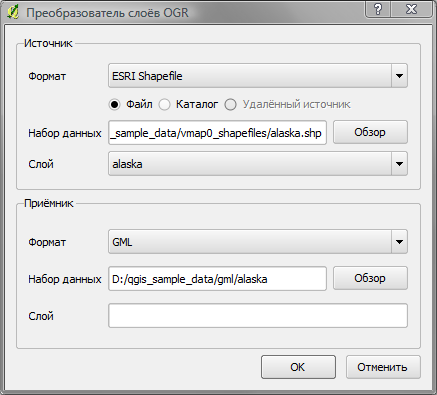
\includegraphics[clip=true, width=9cm]{ogr_converter_dialog}
\end{center}  
\end{figure}

\minisec{Usando el complemento}

\begin{enumerate}
  \item Inicie QGIS, cargue el complemento convertidor de OGR en el administrador de complementos (vea la sección 
  \ref{sec:load_core_plugin}) y haga clic en el ícono \toolbtntwo{ogr_converter}{Conversor de capas OGR} 
 el cual aparece en la barra de menús de QGIS. El complemento conversor de capas OGR aparece como se muestra en la figura \ref{fig:ogrconverter_dialog}.
  \item Seleccione el formato soportado por OGR (e.g., \selectstring{ESRI Shapefile}{\ldots}) y la ruta al archivo vectorial de entrada (ej., \filename{alaska.shp}) en el área de fuente.
  \item Seleccione el formato soportado por ogr (ej., \selectstring{GML}{\ldots}) y defina una ruta y el nombre del archivo vectorial de salida (ej., \filename{alaska.gml}) en el área de destino.
  \item Clic \button{Ok}.
\end{enumerate}

\newpage
